%iffalse
\let\negmedspace\undefined
\let\negthickspace\undefined
\documentclass[journal,12pt,twocolumn]{IEEEtran}
\usepackage{cite}
\usepackage{amsmath,amssymb,amsfonts,amsthm}
\usepackage{algorithmic}
\usepackage{graphicx}
\usepackage{textcomp}
\usepackage{xcolor}
\usepackage{txfonts}
\usepackage{listings}
\usepackage{enumitem}
\usepackage{mathtools}
\usepackage{gensymb}
\usepackage{comment}
\usepackage[breaklinks=true]{hyperref}
\usepackage{tkz-euclide} 
\usepackage{listings}
\usepackage{gvv}                                        
%\def\inputGnumericTable{}                                 
\usepackage[latin1]{inputenc}                                
\usepackage{color}                                            
\usepackage{array}                                            
\usepackage{longtable}                                       
\usepackage{calc}                                             
\usepackage{multirow}                                         
\usepackage{hhline}                                           
\usepackage{ifthen}                                           
\usepackage{lscape}
\usepackage{tabularx}
\usepackage{array}
\usepackage{float}


\newtheorem{theorem}{Theorem}[section]
\newtheorem{problem}{Problem}
\newtheorem{proposition}{Proposition}[section]
\newtheorem{lemma}{Lemma}[section]
\newtheorem{corollary}[theorem]{Corollary}
\newtheorem{example}{Example}[section]
\newtheorem{definition}[problem]{Definition}
\newcommand{\BEQA}{\begin{eqnarray}}
\newcommand{\EEQA}{\end{eqnarray}}
\newcommand{\define}{\stackrel{\triangle}{=}}
\theoremstyle{remark}
\newtheorem{rem}{Remark}
\begin{document}

\bibliographystyle{IEEEtran}
\vspace{3cm}

\title{Question 49, ME Gate 2023}
\author{EE23BTECH11017 - Eachempati Mihir Divyansh$^{*}$}
\maketitle
\newpage
\bigskip

\renewcommand{\thefigure}{\theenumi}
\renewcommand{\thetable}{\theenumi}
\textbf{Question:} Consider the second-order linear differential equation
\[x^2\frac{d^2y}{dx^2}+x\frac{dy}{dx}-y=0, \; x\geq 1\]
with the initial conditions $$y(x=1)=-6,\; \;\; \frac{dy}{dx}\big{|}_{x=1}=2.$$
Then the value of $y$ at $x=2$ is \rule{2cm}{0.1mm}.{\hfill{GATE ME 2023}}\\

\solution
%\fi
\begin{table}[h!]
    \centering
    \begin{tabular}{|m{2cm}|m{2cm}|m{2cm}|}
    \hline
    \textbf{Symbol} & \textbf{Value} & \textbf{Description}\\ [1ex]
    \hline
        $x$ & $x\brak{0}r^4$ & $x\brak{4}$ \\ [1ex]
    \hline
        $y$ & $x\brak{0}r^{10}$ & $x\brak{10}$\\ [1ex]
    \hline
        $z$ & $x\brak{0}r^{16}$ & $x\brak{16}$\\ [1ex]
    \hline
        $r$ & ? & $\frac{x\brak{n}}{x\brak{n-1}}$\\[1ex]
    \hline \vspace{0.1cm}
        $x\brak{0}$ & ? & First term \\[1ex]
    \hline
        $x\brak{n}$ & $x\brak{0}r^nu\brak{n}$ & General Term \\ [1ex]
    \hline
    \end{tabular}

    \caption{Given Information} \label{gateME49.tab:1}
\end{table}

Consider the Mellin Transform
\begin{align}
    y(x)\system{M}\int_{-\infty}^{\infty} x^{v-1}y(x){dx} 
\end{align}
 Let $$Y(v)=\int_{-\infty}^{\infty} x^{v-1}y(x){dx} $$ 
 Properties of the Mellin transform for a system at initial rest include 
\begin{align}
    y'(x) &\system{M} -(v-1)Y(v-1)\\
    xy'(x) &\system{M} -v Y(v)\\
    (x\frac{d}{dx})^ny&\system{M} (-v)^nY(v) 
\end{align}
To modify this, evaluating the Mellin Transform specifically,
\begin{align}
    (x\frac{dy}{dx}) &\system{M} \int_{-\infty}^{\infty} x^{v-1}(x\frac{dy}{dx}){dx}, \;\;x\geq1\\ 
    &\system{M} \int_{1}^{\infty} x^{v}(\frac{dy}{dx}){dx}
\end{align} 
Integrating by parts, 
\begin{align}
    (x\frac{dy}{dx}) &\system{M} [x^v\int \frac{dy}{dx}dx ]\big{|}_1 ^{\infty}-\int_1^{\infty} vx^{v-1}y(x)dx\\
    &\system{M} x^vy(x)\big{|}_1^{\infty} -vY(v)\\
    &\system{M} \lim_{x\rightarrow{\infty}} (x^v y(x))-y(1)-vY(v)
\end{align} 
Let \begin{align} L=\lim_{x\rightarrow{\infty}} (x^v y(x)) \label{gateME49.eq: 10}\end{align}
Subject to $L=0$, from \eqref{gateME49.eq:24}, 
\begin{align}
    (x\frac{dy}{dx}) &\system{M} -y(1)-vY(v)\\
    (x\frac{d}{dx})^2 y &\system {M} v^2Y(v)+vy(1)-y'(1)
\end{align}
The given differential equation can be written as: 
\begin{align}
    x\frac{d}{dx}(x\frac{dy}{dx})&=y,\;\;x\geq 1\\
    \implies (x\frac{d}{dx})^2y&=y,\;\;x\geq 1
\end{align}
Taking Mellin transform on both sides, and from \eqref{gateME49.eq:27} 
\begin{align}
    v^2Y(v)+vy(1)-y'(1)=Y(v),\;\;v<-1
\end{align}
From \tabref{gateME49.tab:1}
\begin{align}
    Y(v)&=v^2Y(v)+6v-2\\
    \implies Y(v)&= \frac{6v-2}{1-v^2}\\&=-\frac{4}{v+1}-\frac{2}{v-1}
\end{align}
Mellin Inversion theorem
\begin{align}
    Y(s) \system{M^{-1}} \frac{1}{2\pi j} \lim_{T \rightarrow \infty}\int_{a-jT}^{a+jT} x^vY(v)dv
\end{align}
Here, there are 2 poles corresponding to $v=1$ and $v=-1$. The limits of integration indicate a contour that can be assumed to cover a plane on eiher side of the verical line $x=a$.
\begin{align}
    y(x)=\frac{1}{2\pi j}\lim_{T\rightarrow \infty} \int_{1-jT}^{1+jT}x^v Y(v)dv 
\end{align}
This can be thought of as a contour encompassing the plane on the left of $x=1$.
Therefore
\begin{align}
    y(x)=\frac{1}{2\pi j}\lim_{T\rightarrow \infty} \int_{1-jT}^{1+jT} \brak{-\frac{4x^v}{v+1}-\frac{2x^v}{v-1}}dv 
\end{align}
By Cauchy's Reidue Theorem
\begin{align}
    y(x)&=-\frac{1}{0!}\lim_{v\rightarrow -1} \brak{v+1} \frac{4x^v}{v+1} - \frac{1}{0!}\lim_{v\rightarrow 1}\brak{v-1} \frac{2x^v}{v-1} \\
    &= -\frac{4}{x} -2x
\end{align}
To find ROC of v, substituting y(x) in \eqref{gateME49.eq: 10}
\begin{align} 
    &\lim_{x\rightarrow \infty} x^v \brak{-2x-\frac{4}{x}}=0\\ \label{gateME49.eq:24}
    \implies& \lim_{x\rightarrow \infty} \brak{4x^{v-1}+2x^{v+1}}=0\\
    \implies& \Re \brak{v+1}<0,\;\Re \brak{v-1}<0\\
    \implies& \Re v<-1\label{gateME49.eq:27}
\end{align}

\begin{figure}[h]
    \centering
    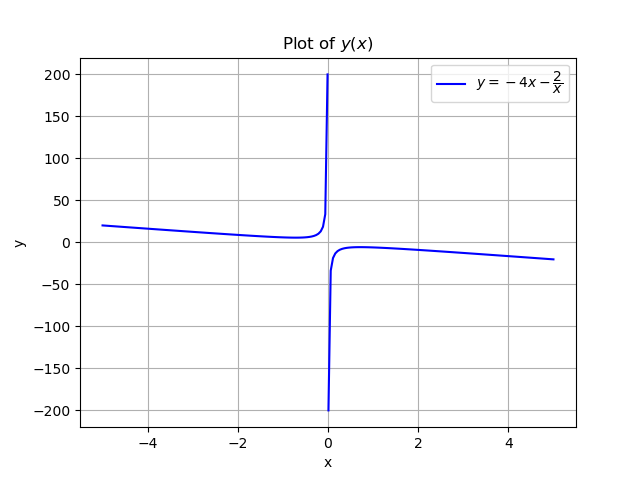
\includegraphics[width=\columnwidth]{figs/fig.png}
    \caption{Plot of $y(x)$ v/s $x$}
\end{figure}

\end{document}
